% ----------------------------------------------------------------
% Report Class (This is a LaTeX2e document)  *********************
% ----------------------------------------------------------------
\documentclass[11pt]{report}
\usepackage[english]{babel}
\usepackage{amsmath,amsthm}
\usepackage{amsfonts}
\usepackage{amssymb}%
\usepackage{graphicx}%
\usepackage{tabularx}
\usepackage{epstopdf}

\addtolength{\textheight}{3.2cm}
\addtolength{\textwidth}{1.5cm}
\addtolength{\marginparwidth}{-2.2cm}
\addtolength{\oddsidemargin}{-1.2cm}
\addtolength{\headheight}{-2.4cm}
%\addtolength{\footskip}{-6cm}

% THEOREMS -------------------------------------------------------
\newtheorem{thm}{Theorem}[chapter]
\newtheorem{cor}[thm]{Corollary}
\newtheorem{lem}[thm]{Lemma}
\newtheorem{prop}[thm]{Proposition}
\theoremstyle{definition}
\newtheorem{defn}[thm]{Definition}
\theoremstyle{remark}
\newtheorem{rem}[thm]{Remark}
% ----------------------------------------------------------------
\begin{document}

%\title{STATS 782, 2017}
\setlength\extrarowheight{3pt}
\begin{tabular*}{\textwidth}{ @{} l @{\extracolsep\fill} c @{\extracolsep\fill} r @{}}
  \hline
  % after \\: \hline or \cline{col1-col2} \cline{col3-col4} ...
  \textbf{STATS 782, 2017} & \textbf{Assignment1} & \textbf{Date: 2017-08-15} \\
   & Zhi Zhang, 708439475, zzha822 & \\
  \hline
\end{tabular*}
%\author{Zhi Zhang, $\ $708439475, $\ $zzha822
%\\The University of Auckland}
%\date{August 3, 2017}
%\maketitle

\begin{enumerate}
    \item[1.] The answers are below:
    \begin{verbatim}> fib = function(n) {
+   s = numeric(n)
+
+   if (n <= 1) s[n] = 0
+   else {
+     s[1:(n - 1)] = fib(n - 1)
+     if (n == 2) s[n] = 1
+     else s[n] = s[n - 1] + s[n - 2]
+   }
+
+   s
+ }
>
> fib(1)
[1] 0
> fib(2)
[1] 0 1
> fib(3)
[1] 0 1 1
> fib(10)
 [1]  0  1  1  2  3  5  8 13 21 34\end{verbatim}

    \item[2.] The answers are below:
    \begin{enumerate}
    	\item[(a)] \begin{verbatim}> clusters.medians = function(x, c) {
+   lenc = length(c)
+
+   d = outer(c, x, function(cj, xi) abs(xi - cj))
+   d.minnum = apply(d, 2, which.min)
+
+   con = outer(1:lenc, d.minnum, function(num, minnum) num == minnum)
+
+   xv = unlist(apply(con, 1, function(t) median(x[t])))
+   xv
+ }
>
> find.clusters.medians = function(x, c) {
+   ctmp1 = c
+   repeat {
+     ctmp2 = clusters.medians(x, ctmp1)
+     if (all(abs(ctmp1 - ctmp2) < 1e-07)) break
+     else ctmp1 = ctmp2
+   }
+   ctmp1
+ }
>
> x = faithful$eruptions
> find.clusters.medians(x, c(2,4))
[1] 1.9830 4.3415\end{verbatim}
 	\item[(b)] \begin{verbatim}> find.clusters.medians(x, c(2,3,4))
[1] 1.9830 3.9665 4.5330\end{verbatim}
 	\item[(c)] \begin{verbatim}> find.clusters.medians(x, c(2,3,4,5))
[1] 1.967 3.600 4.150 4.600\end{verbatim}
    \end{enumerate}

    \item[3.] The answers are below:
    \begin{verbatim}> sign.matrix = function(x) outer(x, x, function(x1, x2) sign(x1 - x2))
>
> conc = function(x, y) {
+   conc.mtx = sign.matrix(x)
+   conc.mty = sign.matrix(y)
+   conc.z = conc.mtx + conc.mty
+   c = length(which(conc.z < 0 | conc.z > 0))
+   n = length(x)
+   c / (n * (n - 1))
+ }
>
> conc(x = 1:5, y = c(3, 1, 4, 5, 2))
[1] 0.6
>
> set.seed(782)
> x = round(rnorm(1000))
> y = x + round(rnorm(1000))
> conc(x, y)
[1] 0.8518939\end{verbatim}
 	
    \item[4.] The answers are below:
    \begin{enumerate}
    	\item[(a)] \begin{verbatim}> nba.df = read.csv("https://raw.githubusercontent.com/zzdxzhangzhi/assignments/master/782/NBA2016-2017.csv",
+ stringsAsFactors = FALSE)
> names(nba.df) = c("team1", "team2", "wins")
> head(nba.df)
          team1               team2 wins
1 Atlanta Hawks      Boston Celtics    2
2 Atlanta Hawks       Brooklyn Nets    2
3 Atlanta Hawks   Charlotte Hornets    1
4 Atlanta Hawks       Chicago Bulls    3
5 Atlanta Hawks Cleveland Cavaliers    3
6 Atlanta Hawks    Dallas Mavericks    2
> 
> nba.names = nba.df$team1[seq(1, 870, length = 30)]
> nba.names
 [1] "Atlanta Hawks"          "Boston Celtics"         "Brooklyn Nets"          
"Charlotte Hornets"      "Chicago Bulls"         
 [6] "Cleveland Cavaliers"    "Dallas Mavericks"       "Denver Nuggets"         
"Detroit Pistons"        "Golden State Warriors" 
[11] "Houston Rockets"        "Indiana Pacers"         "Los Angeles Clippers"   
"Los Angeles Lakers"     "Memphis Grizzlies"     
[16] "Miami Heat"             "Milwaukee Bucks"        "Minnesota Timberwolves" 
"New Orleans Pelicans"   "New York Knicks"       
[21] "Oklahoma City Thunder"  "Orlando Magic"          "Philadelphia 76ers"     
"Phoenix Suns"           "Portland Trail Blazers"
[26] "Sacramento Kings"       "San Antonio Spurs"      "Toronto Raptors"        
"Utah Jazz"              "Washington Wizards"    
> 
> log.likelihood.r = function(r, times, s) {
+   rn = s - sum(r)
+   rr = c(r, rn)
+   
+   if (all(rr > 0)) {
+     mtx = outer(rr, rr, function(ri, rj) ri / (ri + rj))
+     rankv = log(c(mtx[which(row(mtx) != col(mtx))]))
+     sum(times * rankv)
+   } else {
+     -Inf
+   }
+ }
> 
> s = 1000
> Q = function(r) {
+   -log.likelihood.r(r, nba.df$wins, s)
+ }
> 
> count = length(nba.names)
> result = optim(rep(33, count - 1), Q, method = "BFGS")
> result
$par
 [1] 26.967630 15.823522 91.534764 37.369244 29.370856 17.323249 
41.610028 29.444655 35.470375  6.070289 13.160359 28.443720
[13] 16.300844 61.231229 24.235718 28.915184 27.769763 45.295384 
39.273467 48.952031 20.023588 54.466951 57.834409 68.682310
[25] 27.749761 43.350332  9.272344 17.788711 16.557164

$value
[1] 761.4918

$counts
function gradient 
     102       95 

$convergence
[1] 0

$message
NULL

> 
> ratio = 100 / result$par[which.max(result$par)]
> r.value = result$par * ratio
> rr.value = c (r.value, (s - sum(result$par)) * ratio)
> rr.value
 [1]  29.461626  17.286899 100.000000  40.825193  32.087105  18.925323  
45.458169  32.167729  38.750715   6.631676  14.377443
[12]  31.074227  17.808365  66.893961  26.477064  31.589292  30.337942  
49.484352  42.905520  53.479169  21.875391  59.504115
[23]  63.182999  75.034126  30.316089  47.359419  10.129861  19.433831  
18.088389  21.535119
> 
> rank.table = cbind(data.frame(nba.names), rr.value, stringsAsFactors = FALSE)
> ordered.rank = rank.table[order(rank.table$rr.value, decreasing = TRUE),]
> colnames(ordered.rank) = c("name", "rank")
> rownames(ordered.rank) = 1:30
> ordered.rank
                     name       rank
1           Brooklyn Nets 100.000000
2            Phoenix Suns  75.034126
3      Los Angeles Lakers  66.893961
4      Philadelphia 76ers  63.182999
5           Orlando Magic  59.504115
6         New York Knicks  53.479169
7  Minnesota Timberwolves  49.484352
8        Sacramento Kings  47.359419
9        Dallas Mavericks  45.458169
10   New Orleans Pelicans  42.905520
11      Charlotte Hornets  40.825193
12        Detroit Pistons  38.750715
13         Denver Nuggets  32.167729
14          Chicago Bulls  32.087105
15             Miami Heat  31.589292
16         Indiana Pacers  31.074227
17        Milwaukee Bucks  30.337942
18 Portland Trail Blazers  30.316089
19          Atlanta Hawks  29.461626
20      Memphis Grizzlies  26.477064
21  Oklahoma City Thunder  21.875391
22     Washington Wizards  21.535119
23        Toronto Raptors  19.433831
24    Cleveland Cavaliers  18.925323
25              Utah Jazz  18.088389
26   Los Angeles Clippers  17.808365
27         Boston Celtics  17.286899
28        Houston Rockets  14.377443
29      San Antonio Spurs  10.129861
30  Golden State Warriors   6.631676
>  \end{verbatim}
 	    \item[(b)] \begin{verbatim}\end{verbatim}
 	    \item[(c)] \begin{verbatim}> ranks = c(result$par, s - sum(result$par))
> ranks.sort = sort(ranks, decreasing = TRUE)
> first2 = which(ranks == ranks.sort[1:2])
> Q2 = function(r1, r2) {
+   m = max(length(r1), length(r2))
+   if (length(r1) < m)
+     r1 = rep(r1, length = m)
+   if (length(r2) < m)
+     r2 = rep(r1, length = m)
+   
+   ans = numeric(m)
+   for (i in 1:m) {
+     ranks[first2] = c(r1[i], r2[i])
+     ans[i] = -log.likelihood.r(ranks[-length(ranks)], nba.df$wins, s)
+   }
+   
+   ans
+ }
> 
> r1 = seq(50, 100, length = 61)
> r2 = seq(20, 70, length = 61)
> z = outer(r1, r2, Q2)
> contour(r1, r2, z,
+         xlab = paste("rank of", nba.names[first2[1]]),
+         ylab = paste("rank of", nba.names[first2[2]]))
> \end{verbatim}
    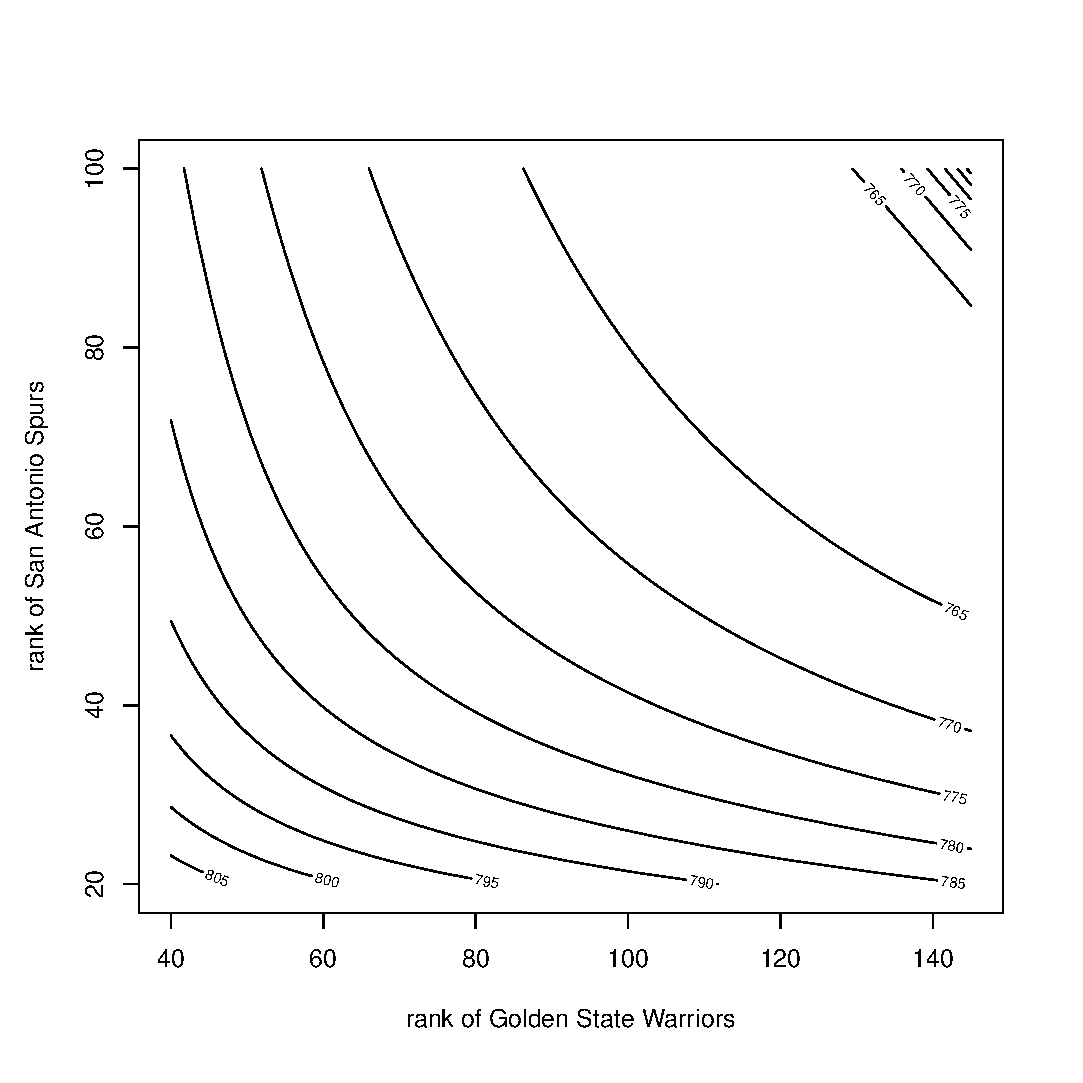
\includegraphics[width=\textwidth]{a2_contour.eps}
    \end{enumerate}

\end{enumerate}

\end{document}
% ----------------------------------------------------------------
